\documentclass[a4paper]{article}
\usepackage{ctex}
\usepackage[affil-it]{authblk}
\usepackage[backend=bibtex,style=numeric]{biblatex}
\usepackage{amsmath,amsthm,amssymb,amsfonts}
\usepackage{graphicx}
\usepackage{bm}
\usepackage{float}
\usepackage{geometry, subcaption}
\geometry{margin=1.5cm, vmargin={0pt,1cm}}
\setlength{\topmargin}{-1cm}
\setlength{\paperheight}{29.7cm}
\setlength{\textheight}{25.3cm}

\addbibresource{citation.bib}

\begin{document}
% =================================================
\title{微分方程数值解 2026 春夏编程作业四}

\author{曾申昊 3220100701
  \thanks{邮箱: \texttt{3097714673@qq.com}
                            \texttt{或} \texttt{3220100701@zju.edu.cn}}}
\affil{浙江大学}

\date{更新时间: \today}

\maketitle

% ============================================

\section{理论分析}

\par  一个 Runge-Kutta 方法由它的 Butcher 表唯一确定，
讲义上已经给出了 classicalRK、ESDIRK、GaussLegendreRK（$s=2,3$）、Fehlberg45
和 Dormand-Prince45 
相应的 Butcher 表，因此在实现时直接使用这些值即可。
\par 对于 $s=4,5$ 时的 Gauss-Legendre RK 方法，由于讲义上没有给出 Butcher 表，
需要自己进行推导。根据 Gauss-Legendre RK 方法的定义有：
\begin{itemize}
    \item $s=4$ 时\\
    \begin{equation}
        \tilde{P}_4(t)
        = t^4 - 2t^3 + \frac{9}{7}t^2 - \frac{2}{7}t + \frac{1}{70}
    \end{equation}
    \item $s=5$ 时\\
    \begin{equation}
        \tilde{P}_5(t)
        = t^5 - \frac{5}{2}t^4 + \frac{20}{9}t^3 - \frac{5}{6}t^2 + \frac{5}{42}t - \frac{1}{252}
    \end{equation}
\end{itemize}
\par 通过求解多项式的根作为 $c_i$，然后利用 $c_i$ 和 Gauss-Legendre RK 方法的定义来求解 $a_{ij}$ 和 $b_i$。
当然在具体实现中，利用计算机数值求解了 Butcher 表。
\par 另外，对于 classicalRK 和 EmembeddedRK ，由于它们是显式方法，
因此在每一步的计算中，$y_{i}$ 可以依次按顺序直接计算得到。
而对于 ESDIRK ，由于它是隐式方法，因此在每一步的计算中，
需要通过求解一个非线性方程来得到 $y_{i}$:
\begin{equation}
    y_{i} = f\left(U^n + k \sum_{j=1}^{i} a_{ij} y_j,t_n + c_i k\right)
\end{equation}
\par 令$x = U^n + k \displaystyle\sum_{j=1}^{i} a_{ij} y_j$ 有
\begin{equation}
    x - k \sum_{j=1}^{i-1} a_{ij} y_j = ka_{ii}f\left(x,t_n + c_i k\right)
\end{equation}
\par 然后可以将上式改写为一个非线性方程 $F(x) = 0$ 的形式：
\begin{equation}
    F(x) = x - k \sum_{j=1}^{i-1} a_{ij} y_j - ka_{ii}f\left(x,t_n + c_i k\right)
\end{equation}
\par 这里的 $x$ 是一个未知量，可以通过牛顿迭代法来求解，最后得到 $y_i$。
对于 GaussLegendreRK，则需要整体求解一个非线性方程组来得到 $y_{1}, \cdots, y_s$:
\begin{equation}
    \left\{
        \begin{aligned}
            &y_{1} = f\left(U^n + k \sum_{j=1}^{s} a_{1j} y_j,t_n + c_1 k\right) \\
            &y_{2} = f\left(U^n + k \sum_{j=1}^{s} a_{2j} y_j,t_n + c_2 k\right) \\
            &\ldots \\
            &y_{s} = f\left(U^n + k \sum_{j=1}^{s} a_{sj} y_j,t_n + c_s k\right)
        \end{aligned}
    \right.
\end{equation}
\par 令 $x_i = U^n + k \sum_{j=1}^{s} a_{ij} y_j$，
且 $X = (x_1, x_2, \ldots, x_s)^T$ 有
\begin{equation}
    F(X) = \left(
        \begin{aligned}
            &ka_{11}y_1 - ka_{11}f\left(x_1,t_n + c_1 k\right) \\
            &ka_{22}y_2 - ka_{22}f\left(x_2,t_n + c_2 k\right) \\
            &\ldots \\
            &ka_{ss}y_s - ka_{ss}f\left(x_s,t_n + c_s k\right)
        \end{aligned}
    \right)
    = \left(
        \begin{aligned}
            &x_1 - U^n - k \sum_{j=1}^{s} a_{1j} f\left(x_j,t_n + c_1 k\right) \\
            &x_2 - U^n - k \sum_{j=1}^{s} a_{2j} f\left(x_j,t_n + c_2 k\right) \\
            &\ldots \\
            &x_s - U^n - k \sum_{j=1}^{s} a_{sj} f\left(x_j,t_n + c_s k\right)
        \end{aligned}
    \right)
\end{equation}

\section{数值结果}

% ===============================================

\par 下面是各种 RK 方法在 Case 1 中的数值结果，
表格中列出了不同步数 $s$ 和阶数 $p$ 的数值解的误差和 CPU 时间。
可以看到，随着步长 $k$ 的减小，各阶方法的误差相应收敛，
同时 CPU 时间也随着步长的减小而成倍增加。
收敛率计算公式为 $\ln\left(e_{k_1}/{e_{k_2}}\right)/\ln(k_1/k_2)$，其中 $e_k$ 表示步长为 $k$ 时的误差。

\begin{table}[htbp]
    \centering
    \caption{classicalRK 方法 Case 1 的数值结果}
    \begin{tabular}{|c|c|c|c|c|c|c|c|}
        \hline
        步数$s$ & 阶数$p$ & 步长$k$ & $L^1$ 误差  & $L^2$ 误差 & $L^\infty$ 误差 & $L^1$ 收敛率 & CPU时间 \\
        \hline
        4 & 4 & 0.001 & 1.409489753 & 1.104347513 & 1.045979639 & ~ & 0.178426 \\ 
        4 & 4 & 0.0005 & 0.1407709702 & 0.1356409153 & 0.1355717279 & 3.324 &  0.342466\\
        4 & 4 & 0.00025 & 0.01385766873 & 0.01310808935 & 0.01309018555 & 3.344 & 0.67978 \\
        \hline
    \end{tabular}
\end{table}

\begin{table}[htbp]
    \centering
    \caption{ESDIRK 方法 Case 1 的数值结果}
    \begin{tabular}{|c|c|c|c|c|c|c|c|}
        \hline
        步数$s$ & 阶数$p$ & 步长$k$ & $L^1$ 误差  & $L^2$ 误差 & $L^\infty$ 误差 & $L^1$ 收敛率 & CPU时间 \\
        \hline
        4 & 4 & 0.001 &  0.5506497038 & 0.4968657399 & 0.494036748 & ~ & 2.842435 \\ 
        4 & 4 & 0.0005 & 0.1058733211 & 0.1039401896 & 0.1039306656 & 2.378 &  5.068874\\
        4 & 4 & 0.00025 & 0.01170636424 & 0.01144023397 &  0.01143836381 & 3.176 & 9.312098 \\
        \hline
    \end{tabular}
\end{table}

\begin{table}[htbp]
    \centering
    \caption{Gauss-Legendre RK 方法 Case 1 的数值结果}
    \begin{tabular}{|c|c|c|c|c|c|c|c|}
        \hline
        步数$s$ & 阶数$p$ & 步长$k$ & $L^1$ 误差  & $L^2$ 误差 & $L^\infty$ 误差 & $L^1$ 收敛率 & CPU时间 \\
        \hline 
        2 & 4 & 0.001 &  0.438992024 & 0.4042199463 & 0.4028505872 & ~ &  0.891834  \\ 
        2 & 4 & 0.0005 & 0.1015177271 & 0.09900061271 & 0.09898083071 & ~ & 1.77578\\
        2 & 4 & 0.00025 & 0.01134063576 & 0.01114197809 &  0.01114102328 & ~ & 3.252941 \\
        \hline 
        3 & 6 & 0.001 &  0.2748804863 & 0.2451879842 & 0.2433583012 & ~ &  1.825705  \\ 
        3 & 6 & 0.0005 & 0.09379102981 & 0.08930397738 & 0.08921260693 & ~ & 3.663726\\
        3 & 6 & 0.00025 & 0.01067449217 & 0.01055192245 &  0.01055156251 & ~ & 6.604867 \\
        \hline
        4 & 8 & 0.001 &  0.2737833161 &  0.2440690851 & 0.2422254269 & ~ &  2.625908  \\ 
        4 & 8 & 0.0005 & 0.09377753465 & 0.0892873569 & 0.08919581617 & ~ & 5.202558\\
        4 & 8 & 0.00025 & 0.0106743117 & 0.01055167057 &  0.01055131024 & ~ & 10.487512 \\
        \hline
        4 & 8 & 0.001 &  0.2737821612 & 0.2440678783 & 0.2422242009 & ~ &  3.841936  \\ 
        4 & 8 & 0.0005 & 0.0937775303 & 0.08928735145 & 0.08919581066 & ~ & 7.563006\\
        4 & 8 & 0.00025 & 0.01067431176 & 0.01055167062 &  0.0105513103 & ~ & 14.944441 \\
        \hline  
    \end{tabular}
\end{table}

\par 对于 Gauss-Legendre RK 方法，
发现当 $s = 3,4,5$ 时，方法收敛速率都没有达到理论阶数 
$p = 2s$，
误差几乎不变，只有CPU时间随着阶数的增加而增加。
可能是因为 Newton 迭代法的误差导致的，也可能是
因为 $s = 4,5$ 的系数是通过数值求解得到的。

\par 对于两种 Embedded RK 方法，
对于任意的初始步长 $k$， 它们都能够通过自适应调整步长来满足误差要求，
并且很快地拟合出图像。Dormand-Prince54 方法的误差往往比 Fehlberg45 方法更小。
初始步长为 $1$
的情况下，Fehlberg45 方法的误差为 $10^0$ 量级，而 Dormand-Prince54 方法的误差为 $10^{-2}$ 量级。
\begin{figure}[htbp]
    \centering
    \begin{subfigure}{0.4\textwidth}
        \centering
        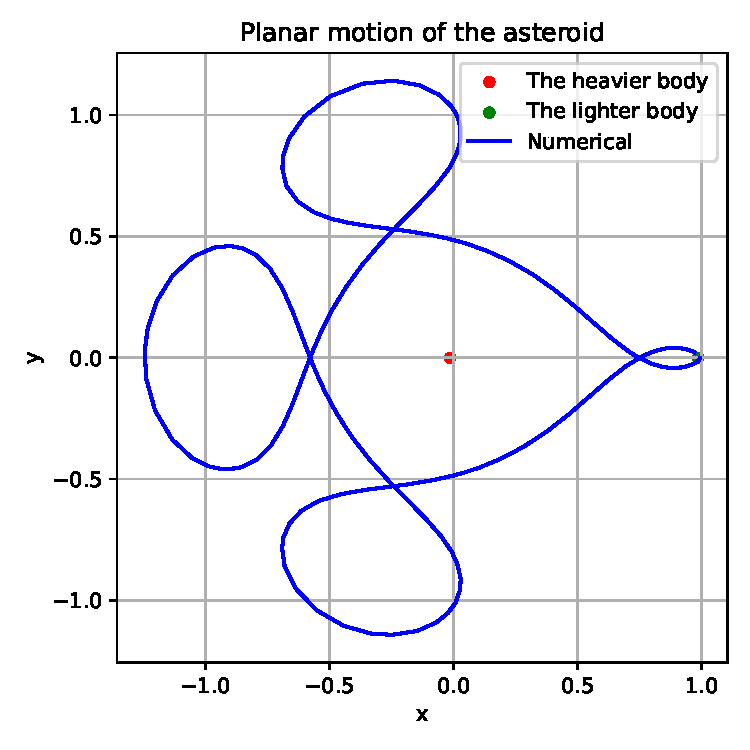
\includegraphics[width=\textwidth]{figure/Fehlberg45.pdf}
        \caption{Fehlberg45 方法的数值解}
    \end{subfigure}
    \begin{subfigure}{0.4\textwidth}
        \centering
        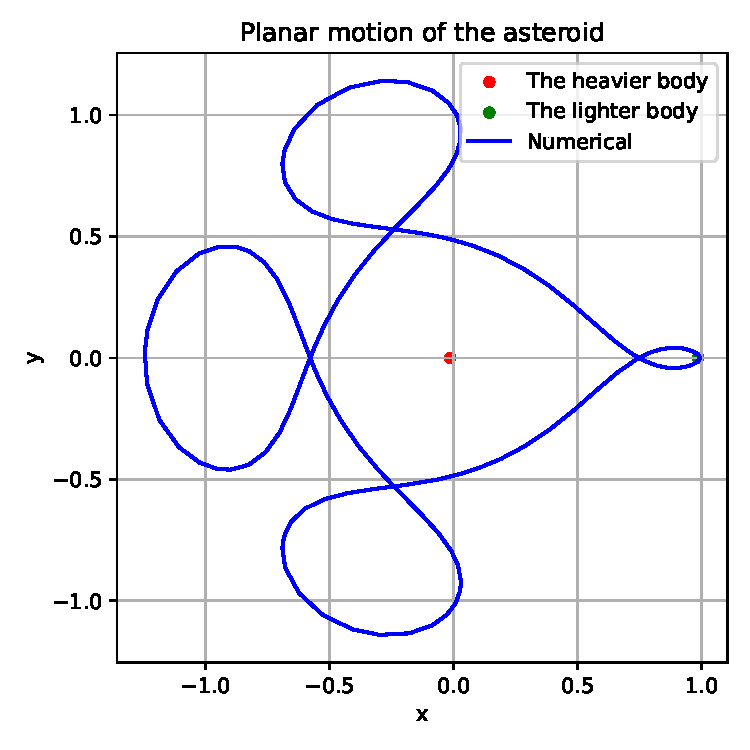
\includegraphics[width=\textwidth]{figure/DormandPrince54.pdf}
        \caption{Dormand-Prince54 方法的数值解}
    \end{subfigure}
    \caption{Embedded RK 方法 Case 1 的数值结果}
\end{figure}

\par Euler 方法固定步数 24000 步，也就是
$k = 17.06521656015796/24000 \approx 0.000711$；
ClassicalRK 方法固定步数 6000 步，也就是
$k = 17.06521656015796/6000 \approx 0.002844$；
以及 Dormand-Prince54 方法调整步数需要改变修正参数 $\rho$，
$\rho_{\text{max}}$ 和 $\rho_{\text{min}}$ 来满足误差要求，前面的
图片大约是150步的结果。
\begin{figure}[htbp]
    \centering
    \begin{subfigure}{0.4\textwidth}
        \centering
        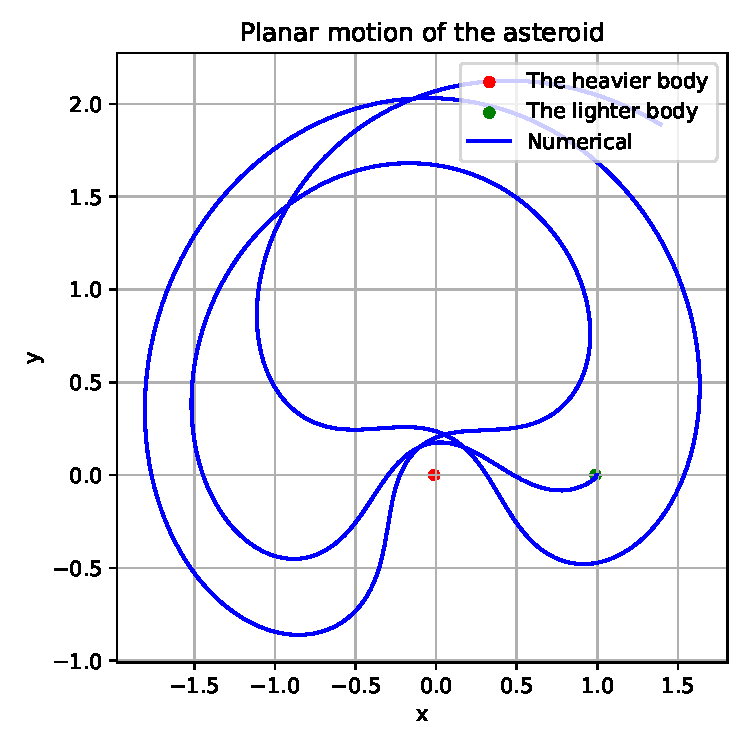
\includegraphics[width=\textwidth]{figure/classicalRK_p1_k0.000711.pdf}
        \caption{Euler 方法在 24000 步时的数值解}
    \end{subfigure}
    \begin{subfigure}{0.4\textwidth}
        \centering
        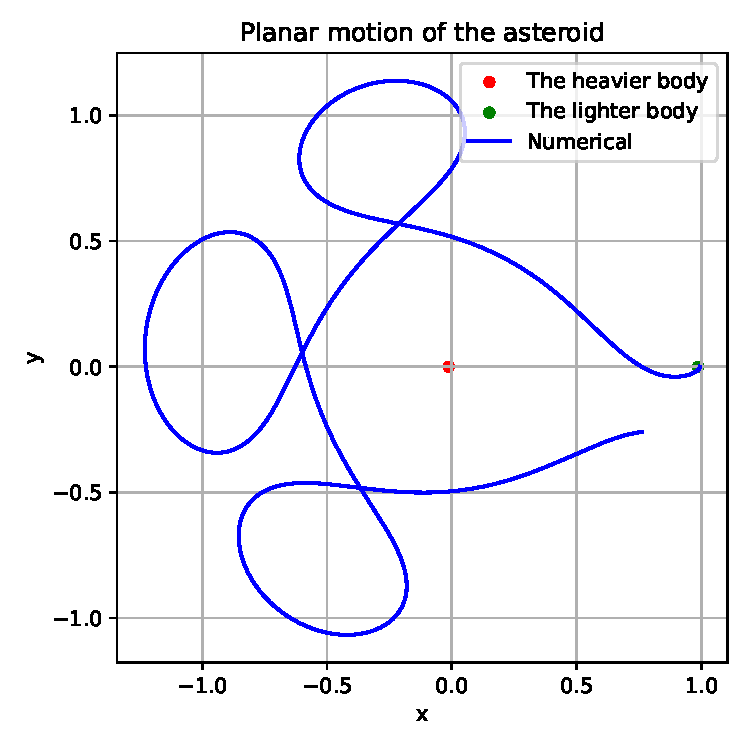
\includegraphics[width=\textwidth]{figure/classicalRK_p4_k0.002844.pdf}
        \caption{ClassicalRK 方法在 6000 步时的数值解}
    \end{subfigure}
    \caption{不同方法 Case 1 的数值结果}
\end{figure}
\par 另外，为了达到 $10^{-3}$ 量级的误差，
Euler 方法在调整到 $k = 10^{-6}$ 时
最大误差为 $0.6475663145$ ， CPU 时间为 $158.2$ 秒，未达到要求；
ClassicalRK 方法在调整到 $k = 2 \times 10^{-5}$ 时，
最大误差为 $0.001085512264$ ， CPU 时间为 $8.5$ 秒，达到了要求；
Dormand-Prince54 方法需要调整参数 $\rho$ 来满足误差要求，
前面的图片大约是150步的结果，最大误差为 $0.04639221339$ 量级， CPU 时间为 $0.00311$ 秒。

\printbibliography

\end{document}